\documentclass[aspectratio=169]{beamer}
\usepackage[utf8]{inputenc}
\usepackage[romanian]{babel}

\usetheme{metropolis}
\usecolortheme{default}
\def\code#1{\texttt{#1}}

%-----------------------------------------------------------------
%This block of code defines the information to appear in the
%Title page
\title[Car Price Predictor Based on Machine Learning]
{\emph{RoCar}: Car Price Predictor Based on Machine Learning}

\subtitle{Lucrare de Licen\c t\u a}

\author
{Huțan Mihai-Alexandru}


\institute[Unibuc]
{
	Facultatea de Matematic\u a-Informatic\u a\\
	Universitatea din Bucure\c sti
}

%End of title page configuration block
%-----------------------------------------------------------------



%-----------------------------------------------------------------
%The next block of commands puts the table of contents at the 
%beginning of each section and highlights the current section:

\AtBeginSection[]
{
	\begin{frame}
		\frametitle{Cuprins}
		\tableofcontents[currentsection]
	\end{frame}
}
%-----------------------------------------------------------------


\begin{document}

%The next statement creates the title page.
\frame{\titlepage}


%--------------------------------------------------------------
%This block of code is for the table of contents after
%the title page
\begin{frame}
	\frametitle{Cuprins}
	\tableofcontents
\end{frame}
%--------------------------------------------------------------

%%%%%%%%%%%%%%%%%%%%%%%%%%%%%%%%%%%%%%%%%%%%%%%%%%%%%%%%%%%%%%%
\section{Ce este \emph{RoCar} și ce îmbunătățiri aduce?}

\begin{frame}{Ce este \emph{RoCar}?}
    \emph{RoCar} este o aplicație web ce permite prezicerea prețurilor mașinilor second-hand folosind o arhitectură multi-modală.\\
    \vspace{10pt}
    \begin{itemize}
        \item Motivație
        \item Obiective
    \end{itemize}
\end{frame}
%--------------------------------------------------------------

\begin{frame}{Îmbunătățiri}
    De-a lungul timpului, diferite abordări au avut loc pentru acest task de regresie, însă atât în literatura de specialitate cât și în serviciile online am regăsit urmoaterele limitări pe care am vrut să le îmbunătățim.
    \vspace{10pt}

    \begin{itemize}
        \item Folosirea exclusivă a datelor structurate.
        \item Ignorarea aspectului estetic al autovehiculelor.
        \item Ignorarea opțiunilor extra.
    \end{itemize}
\end{frame}
%--------------------------------------------------------------

\begin{frame}{Lucrări asociate}
    \begin{itemize}
        \item  Jan ŽIAČIK. “Determinants of Used Car Prices.”, 2023
        \item Svenja Bergmann and Stefan Feuerriegel. “Machine Learning for Predicting Used Car Resale Prices Using Granular Vehicle Equipment Information.”, 2024
        \item Hanqi Su, Binyang Song, and Faez Ahmed. “Multi-modal Machine Learning for Vehicle Rating Predictions Using Image, Text, and Parametric Data.”, 2023
    \end{itemize}
\end{frame}
%--------------------------------------------------------------

%%%%%%%%%%%%%%%%%%%%%%%%%%%%%%%%%%%%%%%%%%%%%%%%%%%%%%%%%%%%%%%
\section{Dezvoltare}

\begin{frame}{Dezvoltare}
    \emph{RoCar} este o aplicație ce are la bază 4 componente distincte și interconectate.

    \begin{itemize}
        \item Scraper: multithreading, scheduler, rezultat %\pause
        \item Core: curățarea și preprocesarea datelor, experimentare %\pause
        \item Backend: performanță, validare, testare, deploy %\pause
        \item Frontend: performanță, deploy
    \end{itemize}
    
\end{frame}
%--------------------------------------------------------------

%%%%%%%%%%%%%%%%%%%%%%%%%%%%%%%%%%%%%%%%%%%%%%%%%%%%%%%%%%%%%%%
\section{Model}

\begin{frame}{Modele folosite}
    În cadrul dezvoltării modelului, am experimentat soluții folosind următoarele modele preantrenate:
    \begin{itemize}
        \item \textbf{BERT}: Bidirectional Encoder Representations from Transformers
        \item \textbf{FastViT}: A Fast Hybrid Vision Transformer using Structural Reparameterization
    \end{itemize}

\end{frame}

\begin{frame}{Experimente}
    Neavând un baseline pe setul de date extras individual, am realizat experimente pentru a dovedi validitatea ideii multimodale.

    \begin{itemize}
        \item \textbf{MLP}
        \item \textbf{FastViT}
        \item \textbf{BERT}
        \item \textbf{Model multi-modal}
    \end{itemize}

\end{frame}
%--------------------------------------------------------------

\begin{frame}{Arhitectura Multimodală}
    \begin{figure}[ht]
    \centering
    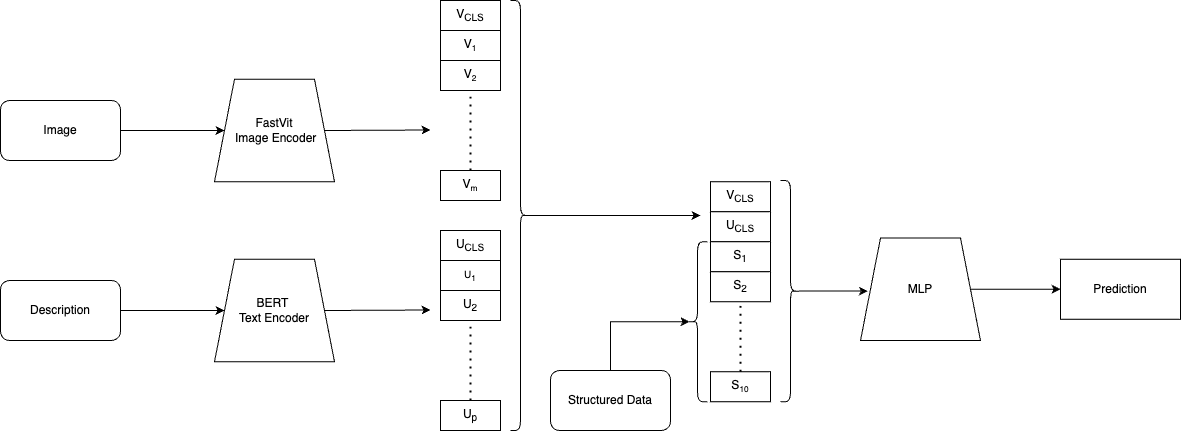
\includegraphics[width=\linewidth]{images/architecture.png}
    \end{figure}
\end{frame}
%--------------------------------------------------------------

\begin{frame}{Rezultate - MAE}
    \begin{figure}
        \centering
        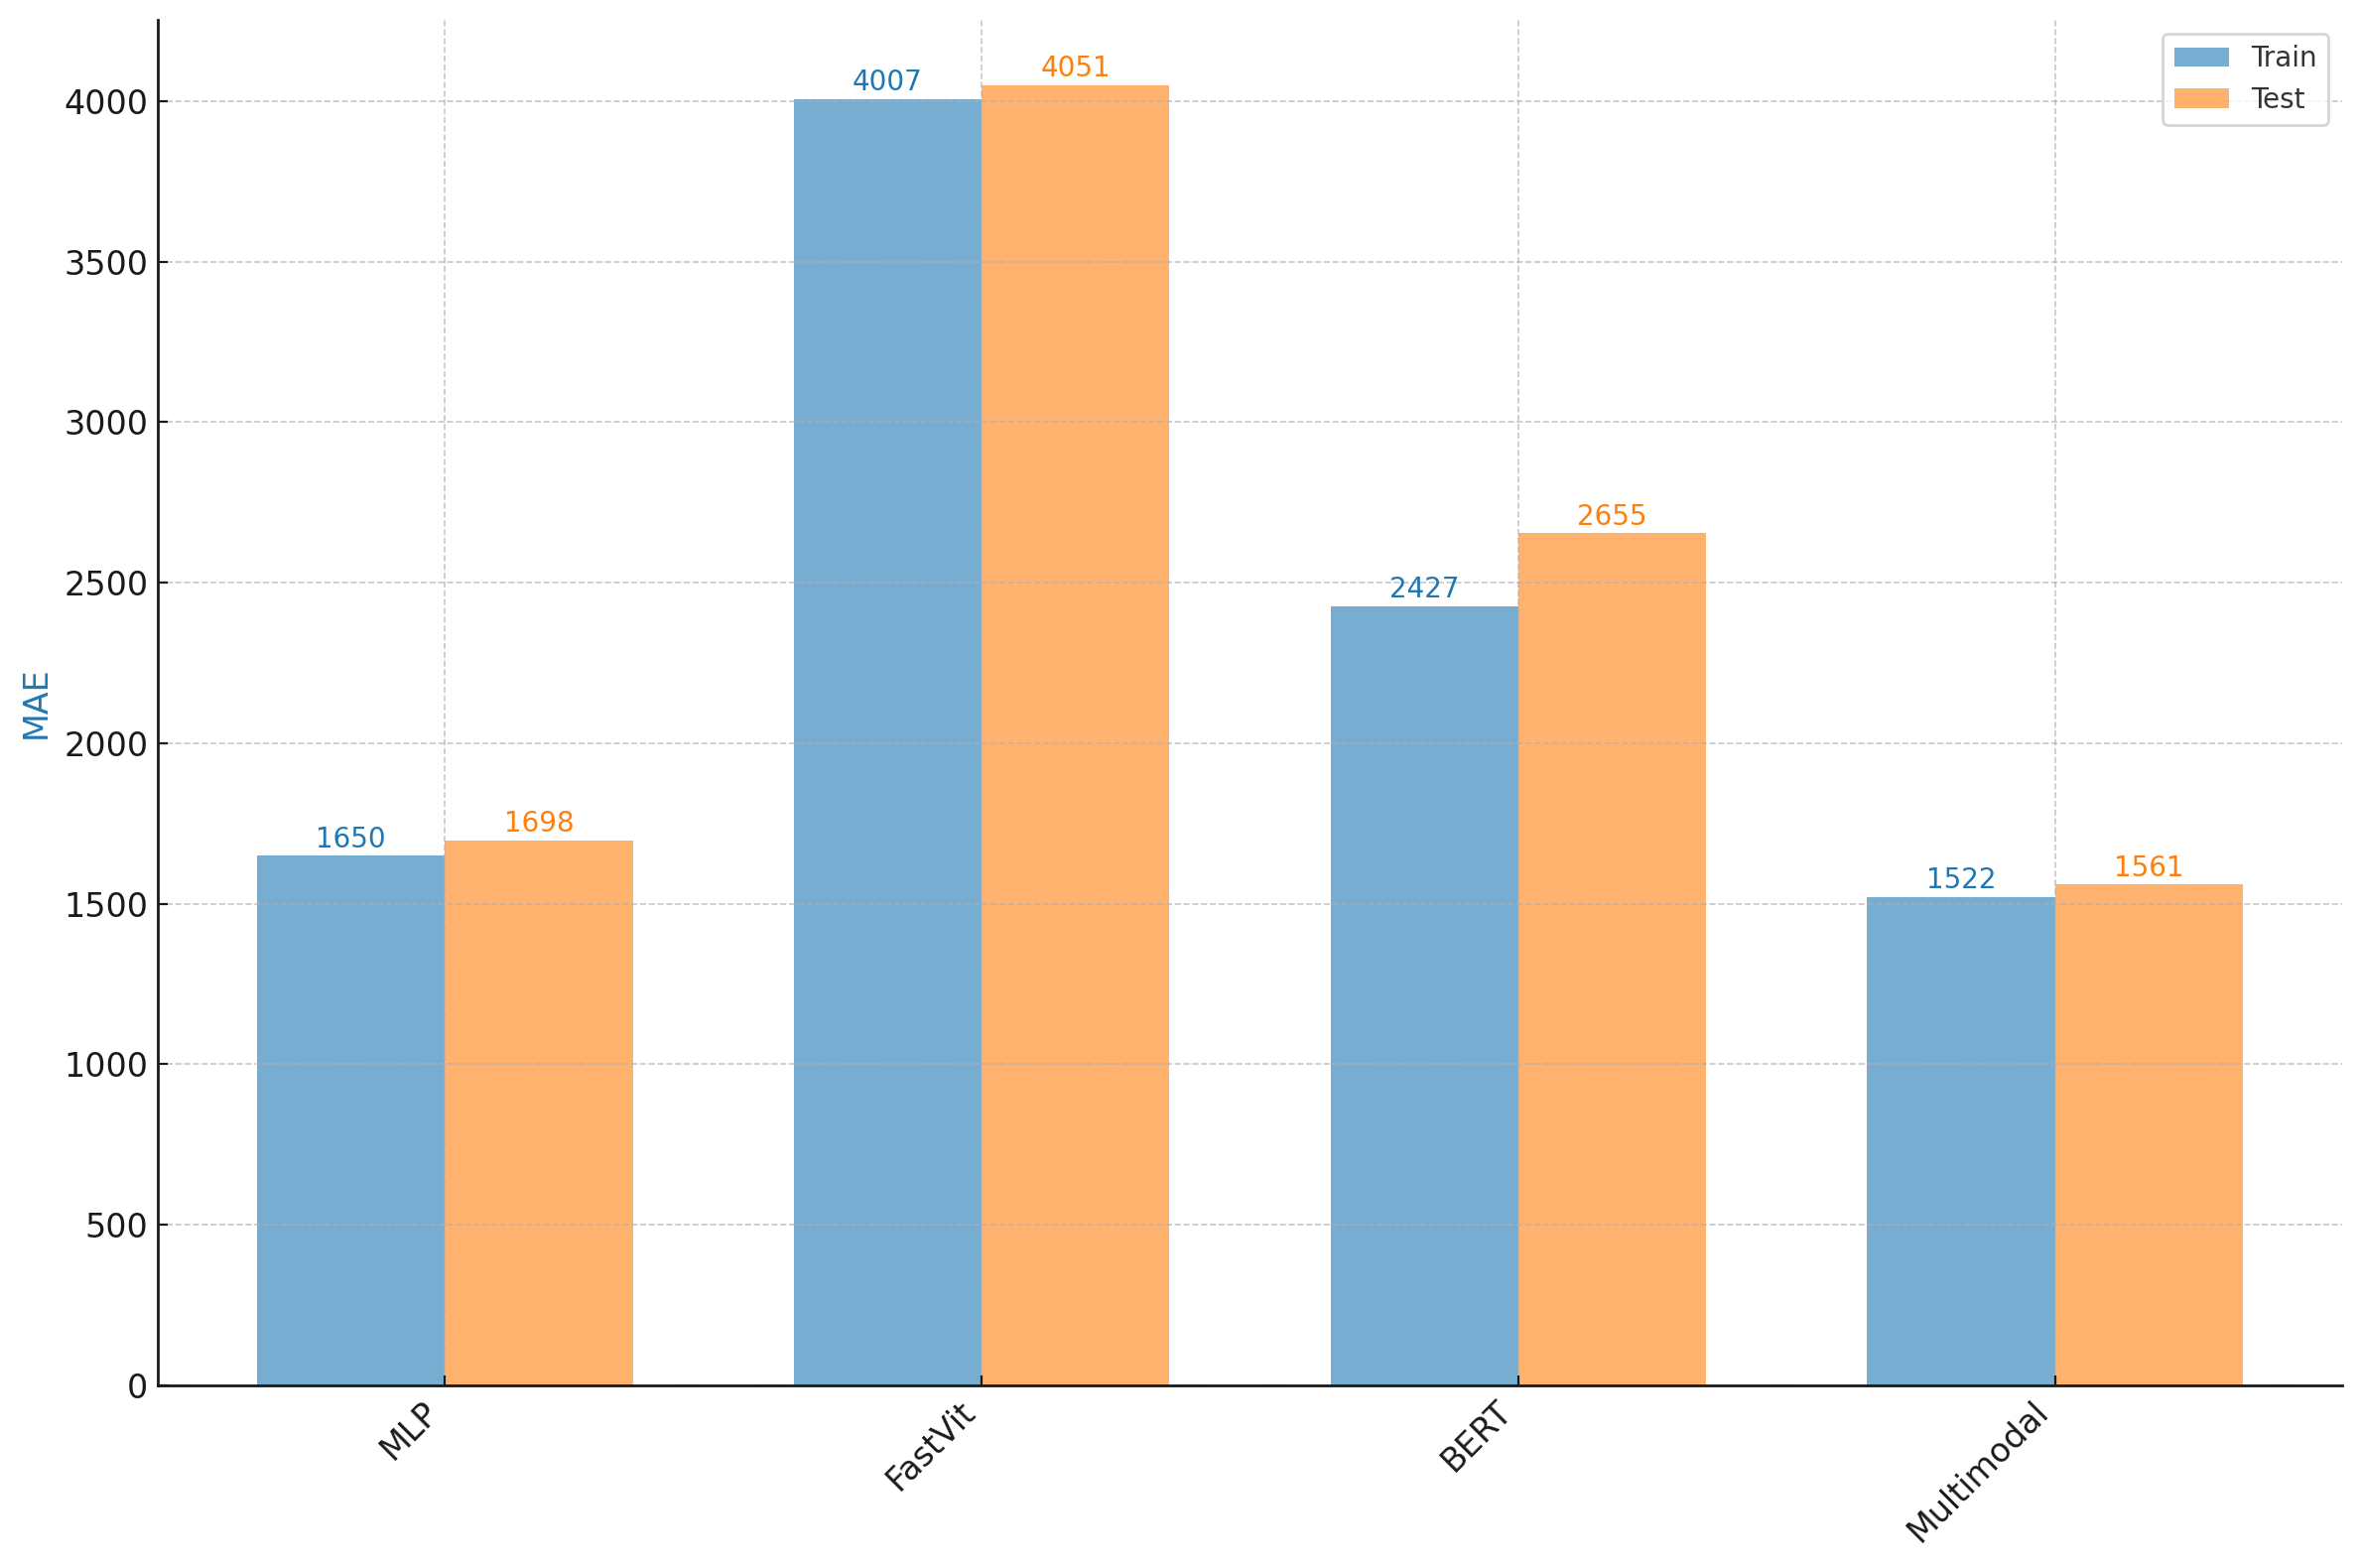
\includegraphics[width=0.8\linewidth]{images/mae.png}
    \end{figure}
\end{frame}

\begin{frame}{Rezultate - R2}
    \begin{figure}
        \centering
        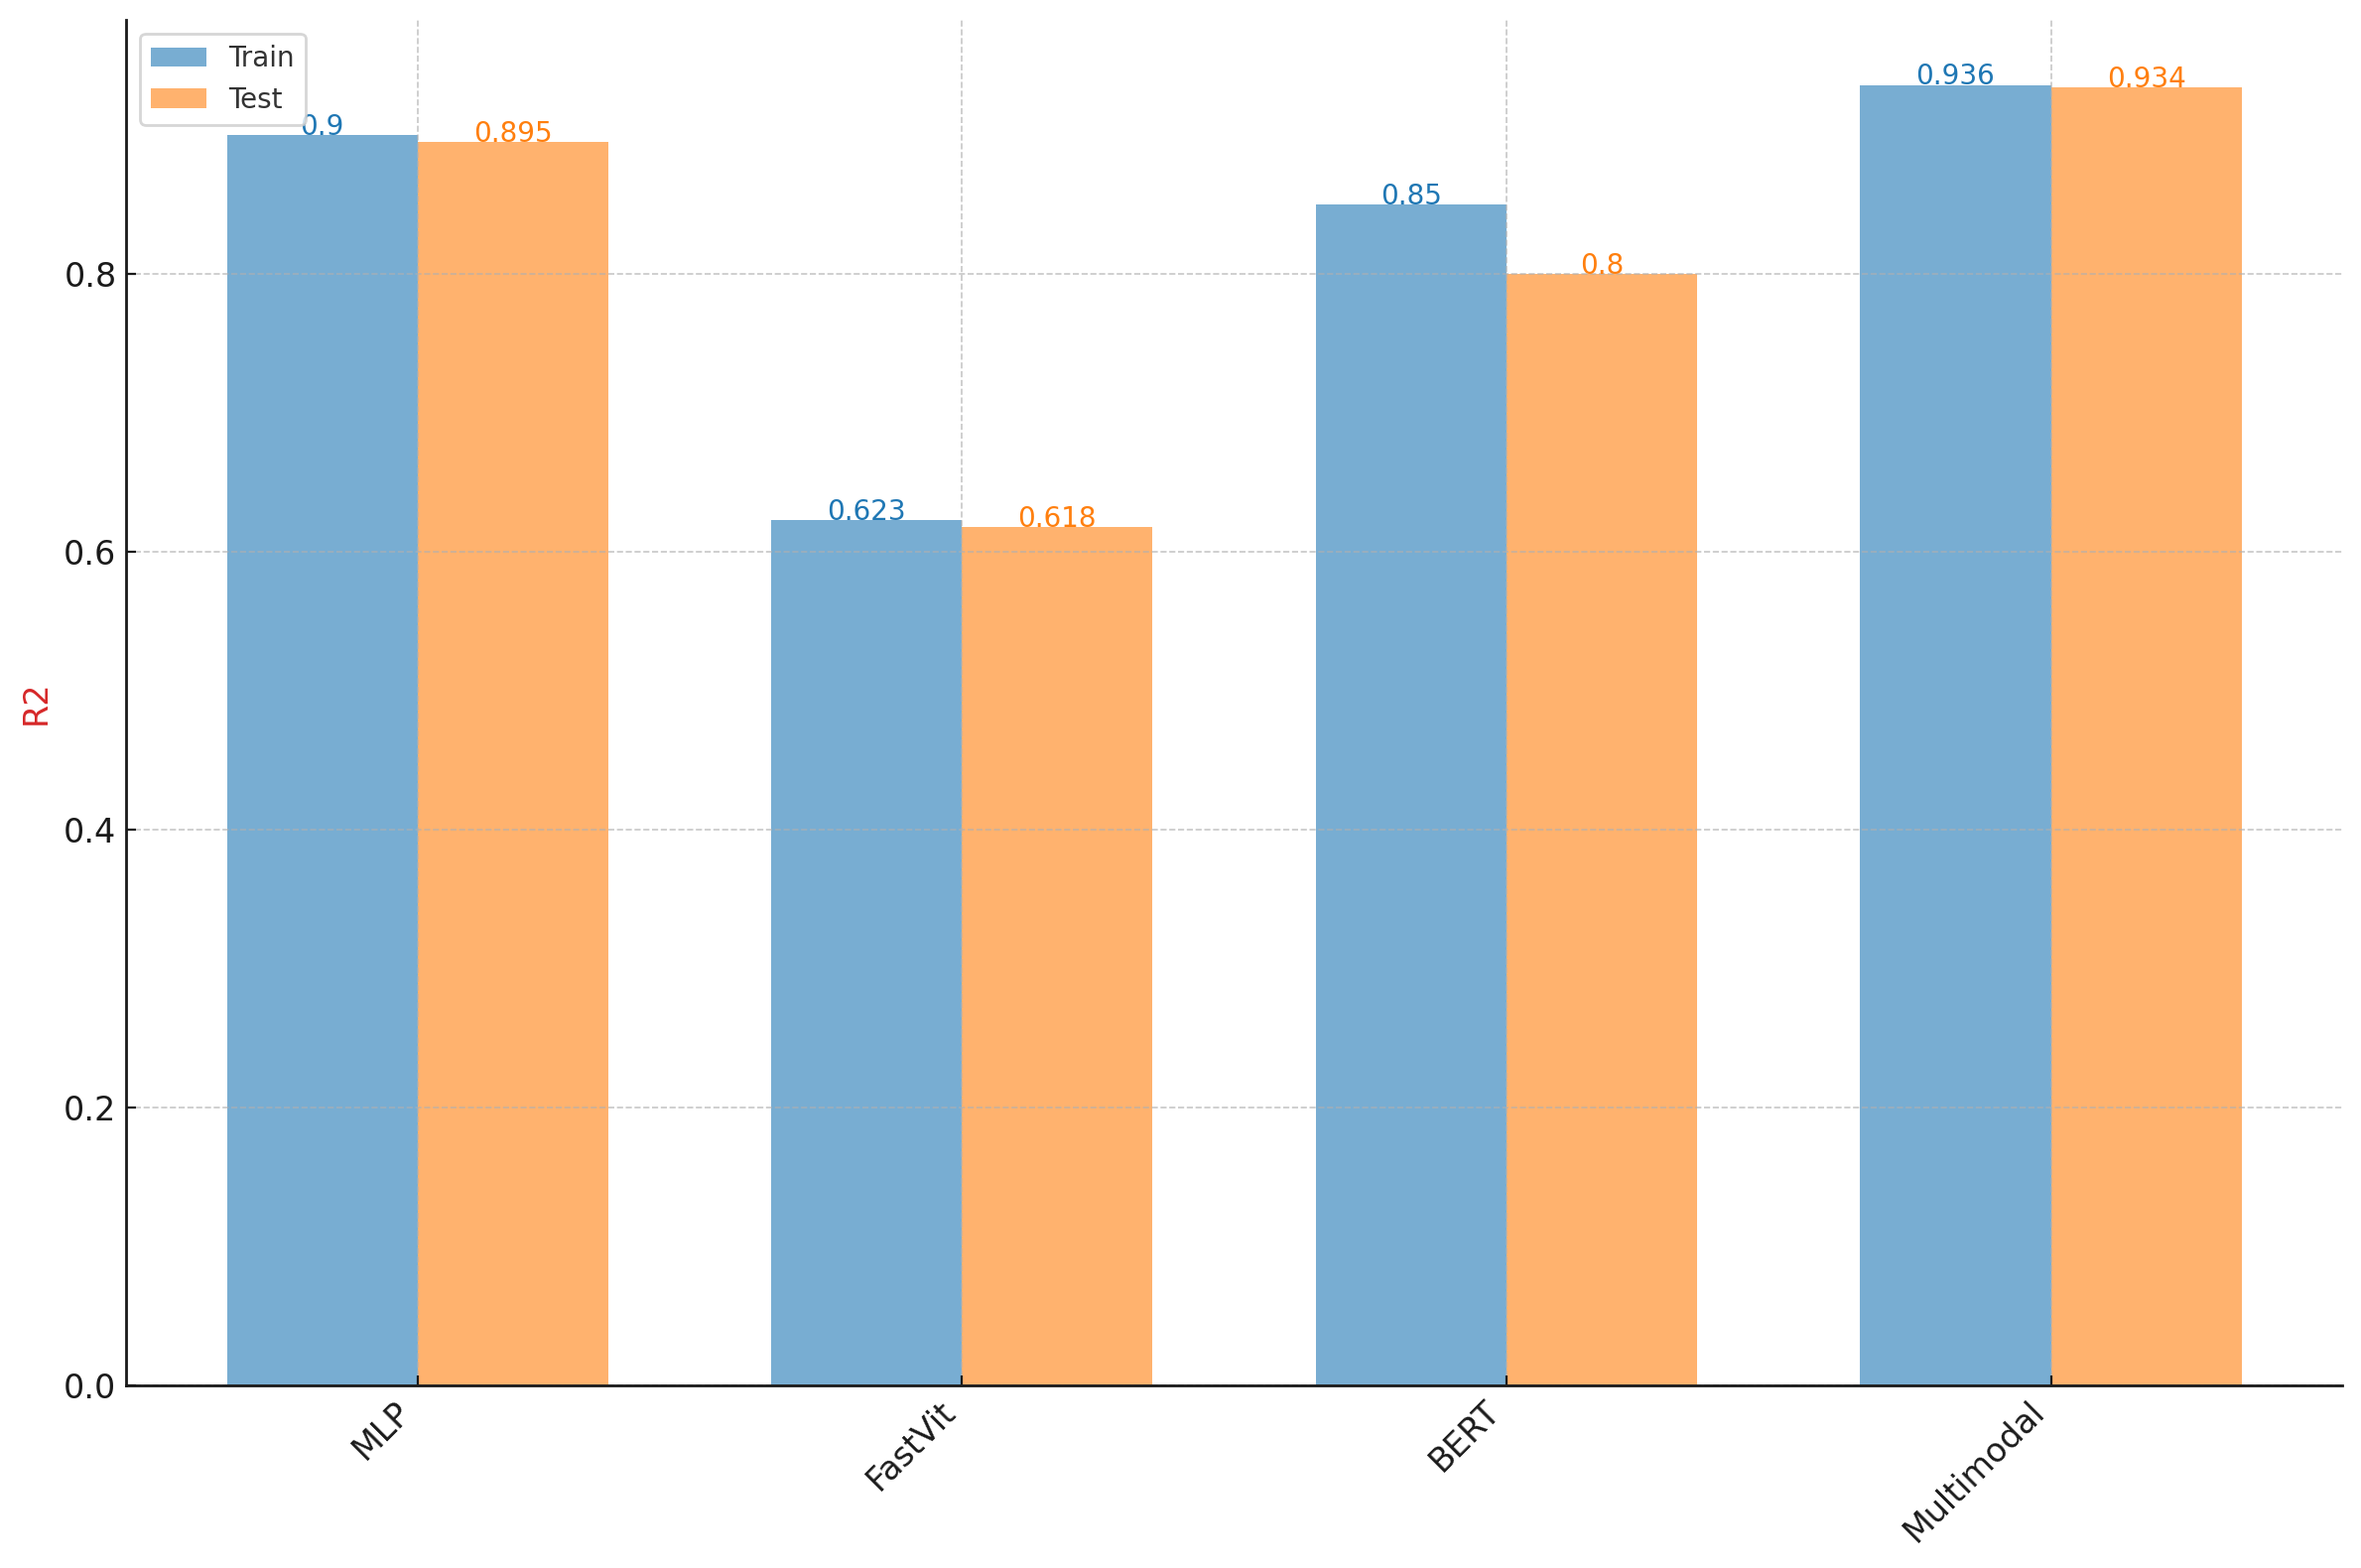
\includegraphics[width=0.8\linewidth]{images/r2.png}
    \end{figure}
\end{frame} 
%--------------------------------------------------------------

%%%%%%%%%%%%%%%%%%%%%%%%%%%%%%%%%%%%%%%%%%%%%%%%%%%%%%%%%%%%%%%
\section{Concluzii}
\begin{frame}{Concluzii}
    \begin{itemize}
        \item Aplicația este într-o stare perfect funcțională și la un nivel "production-ready".
        \item Experimentele realizate au demonstrat ipoteza că în tool-urile și abordările actuale există o pierdere de informație în cadrul pozelor și al descrierilor autoturismelor. 
        \vspace{10pt}
        \item Posibile îmbunătățiri:
        \begin{itemize}
            \item Îmbunătățirea setului de date
            \item Statistici
            \item Un aspect mai plăcut al interfeței
        \end{itemize}
        
    \end{itemize}
    
\end{frame}
%--------------------------------------------------------------

%%%%%%%%%%%%%%%%%%%%%%%%%%%%%%%%%%%%%%%%%%%%%%%%%%%%%%%%%%%%%%%
\section{Demo}

\begin{frame}{Demo}
    \begin{itemize}
        \item Autentificare
        \item Achiziționarea de predicții
        \item Prezicerea prețului unei mașini
        \item Prezentarea interfeței Swagger
    \end{itemize}
\end{frame}
%--------------------------------------------------------------

%%%%%%%%%%%%%%%%%%%%%%%%%%%%%%%%%%%%%%%%%%%%%%%%%%%%%%%%%%%%%%%
\begin{frame}
    \centering
    \textbf{\Huge Întrebări}
\end{frame}
%--------------------------------------------------------------

%%%%%%%%%%%%%%%%%%%%%%%%%%%%%%%%%%%%%%%%%%%%%%%%%%%%%%%%%%%%%%%
\end{document}